\documentclass[tikz]{standalone}
\usepackage{tikz-feynhand}
\usepackage{feynmf}
% bubble diagram
\begin{document}
% bubble diagram
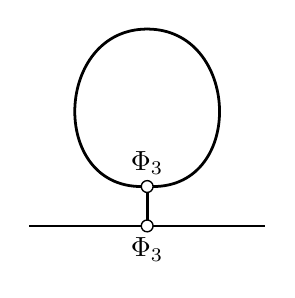
\begin{tikzpicture}
\begin{feynhand}
\vertex[ringdot] (a) at (0,0){}; \vertex[ringdot] (b) at (0,0.5){}; % vertex
\vertex[ringdot] (c) at (0,2.5) ;
\vertex (d) at (1.5,0);\vertex (e) at (-1.5,0); % 両端
\propag[plain,line width = 1pt] (a) to (d);
\propag[plain,line width = 1pt] (e) to (a);
\propag[plain,line width = 1pt] (a) to (b);
\propag[plain,line width = 1pt] (b) to [in=0, out=0, looseness=1.5] (c);
\propag[plain,line width = 1pt] (b) to [in=180, out=180, looseness=1.5] (c);

\node at (-0.0,-0.3) {$\Phi_3$};
\node at (0.0,0.8) {$\Phi_3$};
\end{feynhand}
\end{tikzpicture}
\end{document}

